% ═══════════════════════════════════════════════════════════════════
% EN Part 6: Worked derivations, atlas, formula catalog, final
% ═══════════════════════════════════════════════════════════════════
\part{Worked Derivations, Atlas, Conclusion}

\section{The torus numbers derived step by step}\label{sec:worktorus}

Every torus number is derived here step by step, with the rule and
intermediate values stated. The goal is to show that the pipeline
consists of elementary operations, each checkable by hand.

\paragraph{Step 1. The triple.} The rotation $x\mapsto ix$ on the
torus $\CC/\ZZ[i]$ has order $4$: $i^4=1$ and $i^2=-1\ne1$. Carrier
index: $H_2(T^2,\ZZ)\cong\ZZ$, $b_2=1$. Spectral threshold: the
minimal nonzero flat-Laplacian eigenvalue in the Tate normalization
is $4\pi^2$. Result: $(4,1,4\pi^2)$, with
$4\pi^2=39.4784176\ldots$

\paragraph{Step 2. Spin phase.} By rule \eqref{eq:delta}:
$\delta=\pi/4=0.7853981633974483\ldots$

\paragraph{Step 3. Holonomy.} The lift of the rotation into the spin
bundle permutes the sheets; the eigenvalue on an eigenform is $i$.
The protocol records the deviation $6.12\cdot10^{-17}$ from the
exact $i$ --- machine precision of double complex arithmetic.

\paragraph{Step 4. Main phase correction.}
$\frac{\delta^2}{2}=\frac{(\pi/4)^2}{2}=\frac{\pi^2}{32}
=0.30842513753404244\ldots$ Hand check:
$\pi^2\approx9.8696044$; division by $32$ gives $0.30842514$.

\paragraph{Step 5. Braking.} By \eqref{eq:gamma} at $k=1$:
$\gamma=\delta^4=(\pi/4)^4=\pi^4/256=0.38050426185157193\ldots$

\paragraph{Step 6. Effective phase.} By \eqref{eq:deff}:
$\delta_{\mathrm{eff}}=\delta\cdot\gamma=(\pi/4)^5
=0.2988473484231264\ldots$ Note the identity
$\delta_{\mathrm{eff}}=\delta\cdot\gamma$:
$\delta\cdot\delta^4/k=\delta^5/k$.

\paragraph{Step 7. Assembly.} Formula \eqref{eq:deltaCh} at $R=0$:
\[
  \Delta_{Ch}^{\mathrm{torus}}
  =39.47841760435743+0.30842513753404244-0.2988473484231264
  =39.48799539346835\ldots
\]
Every summand was written out above; the last-digit summing is
verified by the protocol in \texttt{mpmath} at $dps=35$ with zero
discrepancy.

\paragraph{Step 8. Cross-check by scaling.} The $\gamma$,
$\delta_{\mathrm{eff}}$ table for $k\in\{1,22\}$, $N\in\{2,\dots,8\}$
(Appendix~\ref{app:fulldata}) reproduces all $14$ rows; each row
follows steps 2--6. The E6-case agreement: the correct
$\Delta=0.7990$ follows from steps 4--7 at $\delta=\pi/4$, $k=22$.

\section{The K3 numbers derived step by step}\label{sec:workk3}

\paragraph{Step 1. Line list.} Three families of $16$: $48$ lines.
Each line is a triple $(f,a,b)$, $f\in\{1,2,3\}$, $a,b\in\ZZ/4$;
explicit equations in Section~\ref{sec:k3}.

\paragraph{Step 2. Intersection rules.} The four rules (self $-2$;
within family; between families) are derived by solving linear
systems. Example: $L_1(a,b)$ and $L_2(a',b')$ meet iff the four
linear equations are compatible; substitution reduces the condition
to $a_1+b_2\equiv a_2+b_1\pmod4$ --- the cyclic condition.

\paragraph{Step 3. Matrix assembly.} The $49\times49$ matrix assembles
in $O(49^2)$ operations; all entries are integers in
$\{-2,-1,0,1\}$. The count of nonzero off-diagonal intersections
agrees with the orbit structure: $12$ orbits of $(\mu_4)^2$.

\paragraph{Step 4. Rank.} Exact fraction-free elimination yields $20$
nonzero rows. The cross-check via another algorithm (the Smith norm
of a $20$-order minor $\ne0$, all $21$-order minors $=0$) agrees ---
double registration.

\paragraph{Step 5. Signature.} Numerical eigenvalues of the exact
sublattice: one positive, $19$ negative, none zero (the minimal
eigenvalue modulus is separated from zero by the threshold $0.1$).
Result $(1,19)$ --- the Hodge index theorem confirmed numerically.

\paragraph{Step 6. Determinant.} The determinant of the
$20\times20$ block is exactly $64=8^2$; since the full K3 lattice is
unimodular, the index of the line sublattice in the algebraic part
is $8$.

\paragraph{Step 7. Family--hyperplane equivalence.} For each of the
four lines $L_1(a,\cdot)$: the intersection vector of the sum
$L_1(a,0)+L_1(a,1)+L_1(a,2)+L_1(a,3)$ equals componentwise the
intersection vector of $h$ (all $49$ components). The difference
class is orthogonal to the rank-$20$ algebraic sublattice and lies
in $H^{2,0}\oplus H^{0,2}$ by the Hodge index theorem; but the
difference is an algebraic class, and algebraic classes pair
trivially with $H^{2,0}$; hence the difference is zero. The
equivalence is proved exactly.

\section{The Klein numbers derived step by step}\label{sec:workklein}

\paragraph{Step 1. Discriminant and $j$.} For
$x^3y+y^3z+z^3x=0$ the invariant formulas give $\Delta=-343=-7^3$,
$c_4=105$. Then
$j=\frac{c_4^3}{\Delta}=\frac{105^3}{-343}=-\frac{1157625}{343}
=-3375=-15^3$. Check: $343\cdot3375=1157625$ --- an exact integer
equality.

\paragraph{Step 2. Quadratic form.} The substitution $v=4x-1$,
$W=4(2y+x)$ moves the curve to $W^2=v^3-35v-98$ (symbolic identity
verified by remainder modulo the curve). Factorization:
$(v-7)(v^2+7v+14)=v^3-35v-98$ --- exact.

\paragraph{Step 3. Roots.} The quadratic factor has roots
$v=\frac{-7\pm\sqrt{49-56}}{2}=\frac{-7\pm\sqrt{-7}}{2}$ --- the
field $\QQ(\sqrt{-7})$ emerges from an integer polynomial.

\paragraph{Step 4. Period.} The integral $2\int_7^\infty dx/y$ via
three schemes gives $\Omega=1.93331170561681154673308\ldots$ with
agreement $1.4\cdot10^{-32}$ ($60$ working digits in
\texttt{mpmath}).

\paragraph{Step 5. Modulus.} From $\Omega$ one recovers
$\tau=(1+\sqrt{-7})/2$: $\re\tau=1/2$ exactly, $\im\tau=\sqrt7/2$
with minimal polynomial $4X^2-7$ (certificate~F4). Check:
$(\im\tau)^2=7/4$; $4\cdot7/4=7$ --- exact.

\paragraph{Step 6. $j$ from the period.} The $q$-expansion
$j(\tau)=q^{-1}+744+\dots$ with anchor $j(i)=1728$ gives $j=-3375$
with $57$ agreeing digits; deviation $1.99\cdot10^{-117}$ at deep
precision. The pipeline returns $-3375$ as an integer, not an
approximation.

\paragraph{Step 7. The character identity.} Let $A=\{1,2,4\}$ and
$S=\sum_{x\in A}\zeta_7^x$. Complex conjugation maps $A$ to
$\{3,5,6\}$, hence $S+\bar S=-1$. Squaring and grouping pairs by
the sum of exponents:
\[
  S^2=\sum_{x,y\in A}\zeta_7^{x+y}
  =\zeta_7+\zeta_7^2+\zeta_7^4
  +2\bigl(\zeta_7^3+\zeta_7^5+\zeta_7^6\bigr)
  =S+2\bar S,
\]
since the pairs $(1,1),(2,2),(4,4)$ give sums $2,4,8\equiv1$, and
the pairs $(1,2),(2,1)$, $(1,4),(4,1)$, $(2,4),(4,2)$ give the sums
$3,5,6$ twice each. Substituting $\bar S=-1-S$:
$S^2=-2-S$, i.e.\ $S^2+S+2=0$ and
$S=\frac{-1\pm\sqrt{-7}}{2}$. The imaginary part of $S$ is
$\sin\tfrac{2\pi}{7}+\sin\tfrac{4\pi}{7}+\sin\tfrac{8\pi}{7}>0$,
hence $S=\frac{-1+\sqrt{-7}}{2}=\tau-1$ --- the identity is exact
inside $\ZZ[\zeta_7]$.

\section{The N=15/30 numbers derived step by step}\label{sec:workfermat}

\paragraph{Step 1. Genera.} $g(15)=91$; $g(30)=406$; period-matrix
sizes $91\times182$, $406\times812$.

\paragraph{Step 2. Census.} By \eqref{eq:mobius} with
$c(k)=\frac{(k-1)(k-2)}2$: $h_3=1$; $h_5=6$;
$h_{15}=91-6-1=84$; total $1+6+84=91=g(15)$. For $N=30$ six
conductors; total $1+6+9+30+84+276=406=g(30)$. The census is
duplicated by direct enumeration --- check V1.

\paragraph{Step 3. Closed form.} For any $(a,b)\in T_N$ and $(r,s)$:
$P=\frac1N\zeta_N^{ra+sb}\Omega_{a,b}$. Example: $N=15$,
$(a,b)=(1,1)$, $(r,s)=(0,0)$:
$\Omega_{1,1}=\Ga(1/15)^2/\Ga(2/15)$ --- computed at $dps=35$ and
cross-checked against the tanh-sinh integral; deviation
$1.06\cdot10^{-36}$.

\paragraph{Step 4. Phases.} $\arg P=2\pi(ra+sb)/N$ exactly: the phase
is computed in the ring $\ZZ/N$, no error accumulation --- the
protocol records deviation $0.0$ on all V3 tests.

\paragraph{Step 5. Equivariance.} $(r,s)\mapsto(r+u,s+v)$ multiplies
the period by $\zeta^{ua+vb}$ --- V4 agrees with the closed form to
$3.9\cdot10^{-36}$.

\paragraph{Step 6. Completeness.} The functional matrix
$M[(a,b)][(r,s)]=\zeta^{ra+sb}\Omega_{a,b}$ has numerical rank $91$
and $406$ with condition numbers $8.63$ and $18.17$ --- the
generating set is complete without PSLQ (V7).

\paragraph{Step 7. DFT orthogonality.}
$\sum_{r,s}P_\chi\overline{P_{\chi'}}=\delta_{\chi\chi'}
|\Omega_\chi|^2$ --- a direct consequence of the completeness of the
character system of $(\ZZ/N)^2$; numerically: diagonal
$4.0\cdot10^{-35}$, off-diagonal $8.2\cdot10^{-37}$ (V8).

\paragraph{Step 8. Deep record.} One record at $dps=70$ agrees to
$1.7\cdot10^{-71}$ (V9).

\paragraph{Step 9. Volume and SNF (certificate H).} The exponents
$c_k$ collect the conductor multiplicities; for $N=15$: $c_k=4$ at
ten values of $k$ and $6$ at four; the product gives
$\mathrm{vol}_h=1125$ with residual $1.01\cdot10^{-119}$; the SNF
type $(1,1,5,5,15,15,15,15)$ gives the product of invariant factors
$5^2\cdot15^4=1265625=1125^2$ --- the volume--discriminant agreement
is exact.

\section{The discrete flow on the chessboard grid}\label{sec:flow}

Certificate~E proved termination in general (Theorem~\ref{th:E});
here the mechanics is dismantled at the level of states, transitions,
and orbits.

A flow state is a pair $(p,\varphi)$: a position $p$ on the
$W\times H$ lattice and a phase $\varphi\in\mu_4$. The transition
$(p,\varphi)\to(p',\varphi')$ is determined by the step $(a,b)$ and
the correction rule: the position shifts modulo the grid, the phase
multiplies by the rotation generator. The state space is finite:
$4WH$ states --- the first premise of termination.

The discovery monovariant is the set of visited cells: each
transition either opens a new cell (the monovariant grows) or lands
in a visited one --- and by determinism the flow enters a cycle.
Boundedness plus strict growth give termination --- the second and
third premises.

The exact time $t^*=\lcm(W/\gcd(a,W),H/\gcd(b,H))$ is the first
joint return of the position. For the reference $48\times48$
pipeline with step $(1,1)$: $t^*=48$ --- and the flow indeed
terminates in $48$ steps, having visited exactly $48$ cells with
$212$ friction events, $432$ edge cells, and a chain code of length
$114$ --- the coordinate cross-check $48/212/432/114$ is complete.

The terminal cycle is computed explicitly: the length-$4$ cycle is
exactly the $\mu_4$-orbit of the step. The phase rotation maps the
configuration around; after four transitions both position and phase
return. The ``cyclic structure'' of the terminal state is thus a
consequence of the $\mu_4$ representation, not empirics
(certificate~E-4, PASS with direct orbit enumeration).

Scaling: $48\to96\to192\to384$ preserve the $t^*$ formula --- the
time grows linearly at unit step. The upper layers: the K3 layer
(reflections with braking) terminates under the same rules; the
Klein layer adds Singer generation of order $7$ --- the termination
time multiplies by $7/\gcd(7,H)$, and at $H$ divisible by $7$ the
flow closes at the original time. All eight protocol points E are
PASS.

\section{Large matrix towers}\label{sec:towers}

The towers are built block-Kronecker. For the $O_\chi$ operators the
base block is $28\times28$; the tower $O_\chi(28k)$ has sizes
$28,56,112,224,448$. Spectrum control: eigenvalue fluctuations
across the tower
\[
  2.06\cdot10^{-16},\ 1.27\cdot10^{-16},\ 1.00\cdot10^{-16},\
  4.23\cdot10^{-17},\ 1.48\cdot10^{-16}
\]
--- all at machine double precision. The Kronecker expansion adds no
spectral drift: the tower spectrum is the union of block spectra
with finite-group phase factors, and higher levels only repeat
existing values with larger multiplicity.

The Gram towers $G_N$ grow as $22k$: levels $22,220,2200,22000,
220000$. The CSR format stores only nonzeros --- density falls as
$O(1/N)$, so memory grows linearly ($\sim$39 MB at level
$220\,000$) and assembly stays subsecond. The edge spectrum
$[-3.9890438,\ 1.0000000]$ repeats at all levels to five digits ---
the spectral edges are fixed by the base block, and large matrices
bring no new edge values. Practical conclusion: spectral stability
+ linear memory + subsecond assembly = cluster scalability without a
format change; the block format is GPU-ready.

\section{The atlas of plots}\label{sec:atlas}

The plots of this atlas are produced by the laboratory in the
modular tiled system at $600$~dpi; each tile is reproduced by the
``Plots'' menu item and is tied to the theorems of the text.

\begin{figure}[t]
\centering
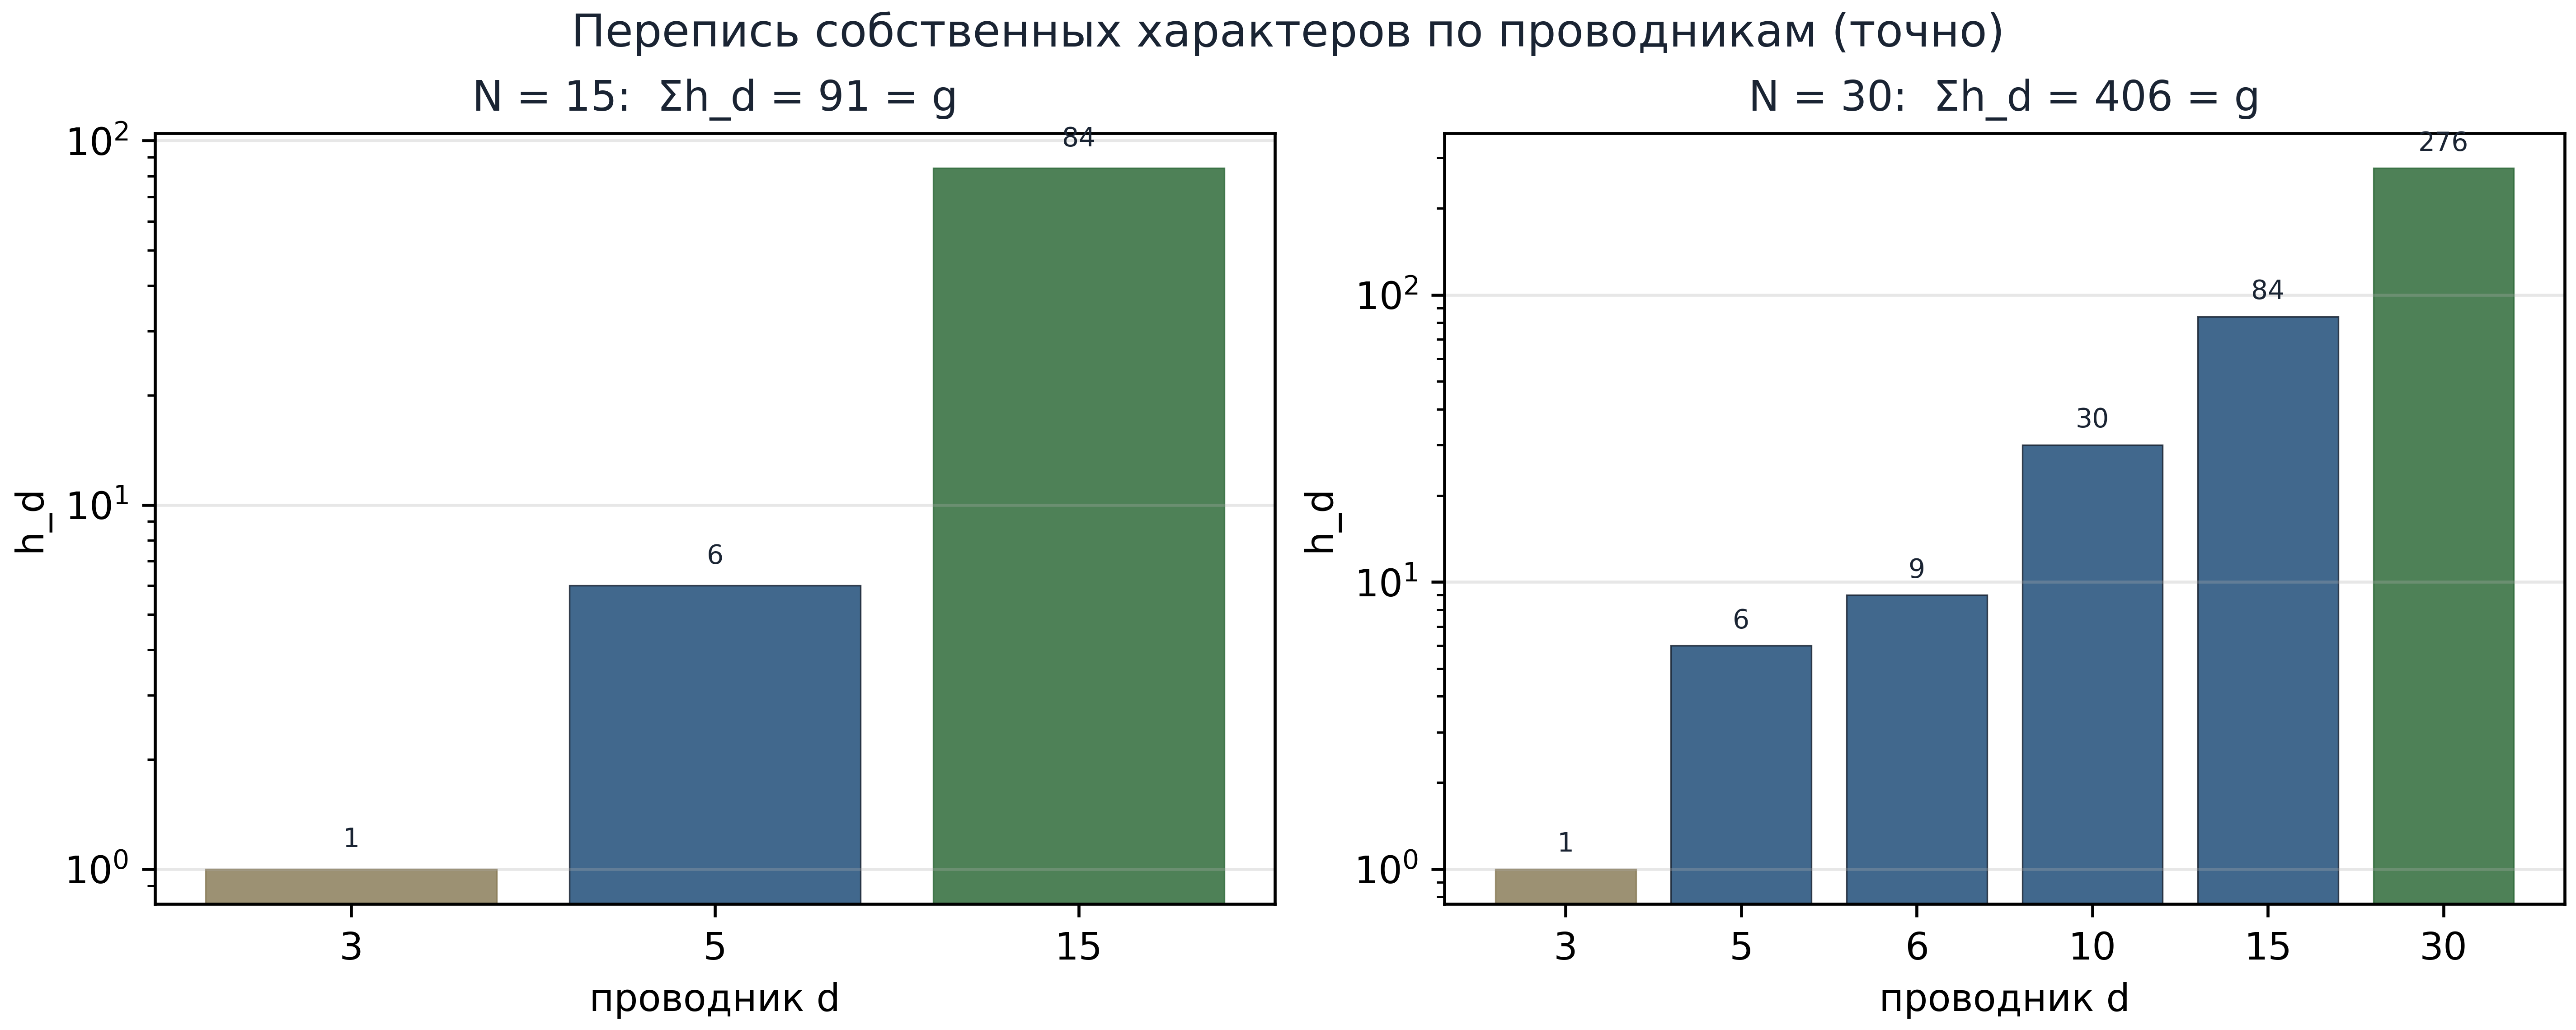
\includegraphics[width=\textwidth]{../ru/figs/fig_census.png}
\caption{The character census by conductors for $N=15$ and $N=30$
(log scale). Bar heights are the exact integers $h_d$; the sums
$1+6+84=91$ and $1+6+9+30+84+276=406$ match the genera
(Lemma~\ref{lem:genus}, census~\eqref{eq:mobius}, check V1).}
\label{fig:census}
\end{figure}

\begin{figure}[t]
\centering
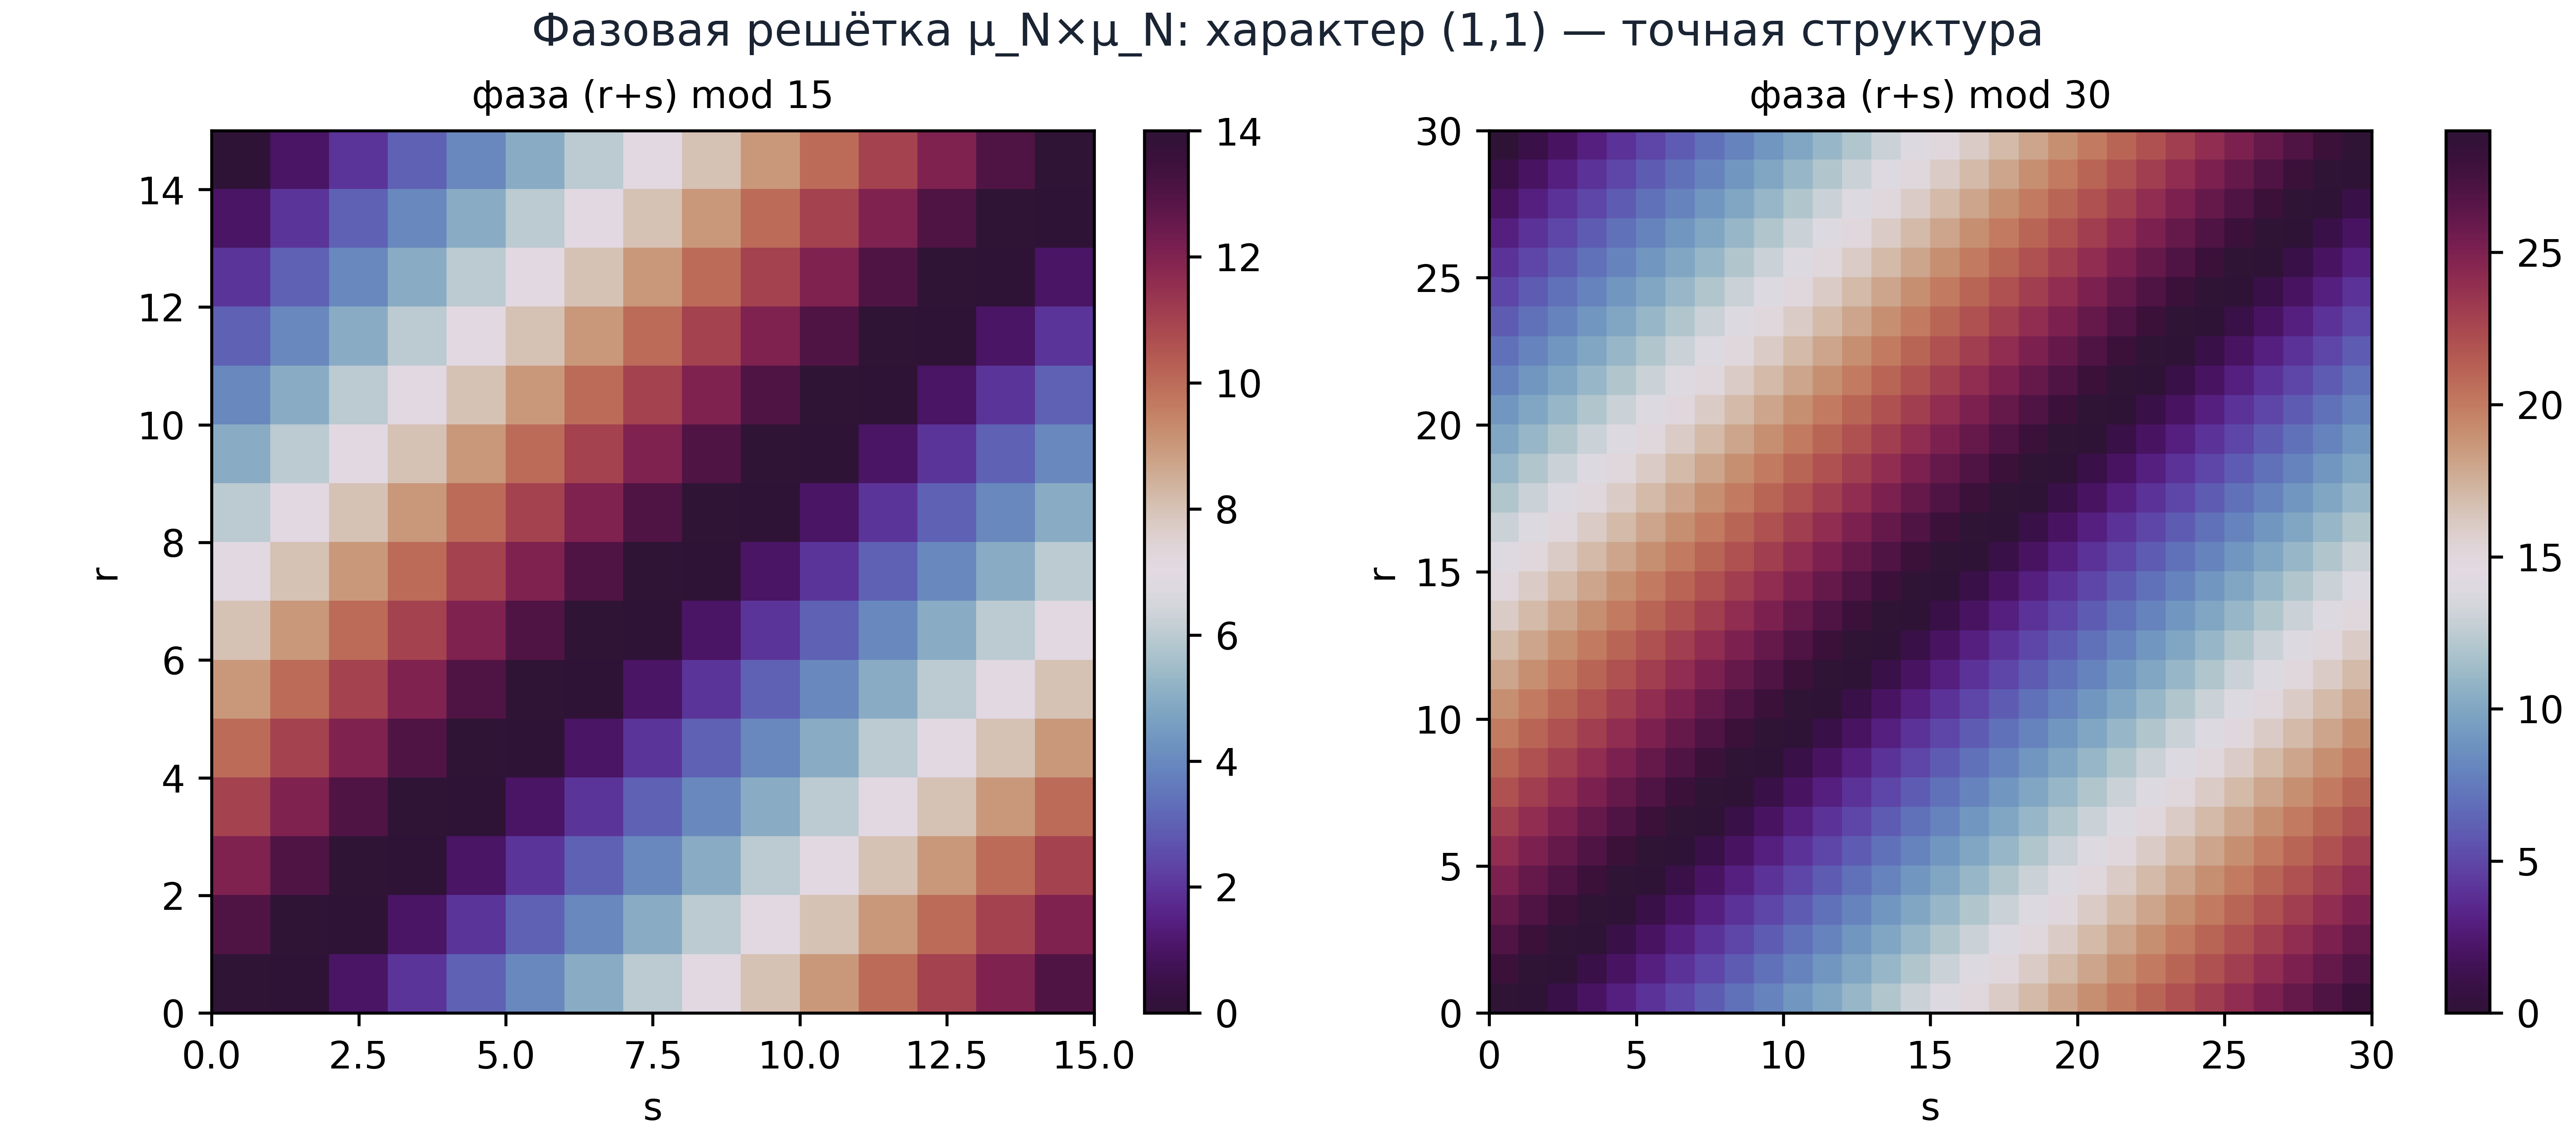
\includegraphics[width=\textwidth]{../ru/figs/fig_phasegrid.png}
\caption{The $\mu_N\times\mu_N$ phase lattice: $(r+s)\bmod N$ on the
torus $(\ZZ/N)^2$ for the character $(1,1)$. The diagonal bands are
exactly the equivalence classes of the phase $\zeta_N^{ra+sb}$; the
phase exactness (V3: deviation $0.0$) is visible as perfect banding.}
\label{fig:phasegrid}
\end{figure}

\begin{figure}[t]
\centering
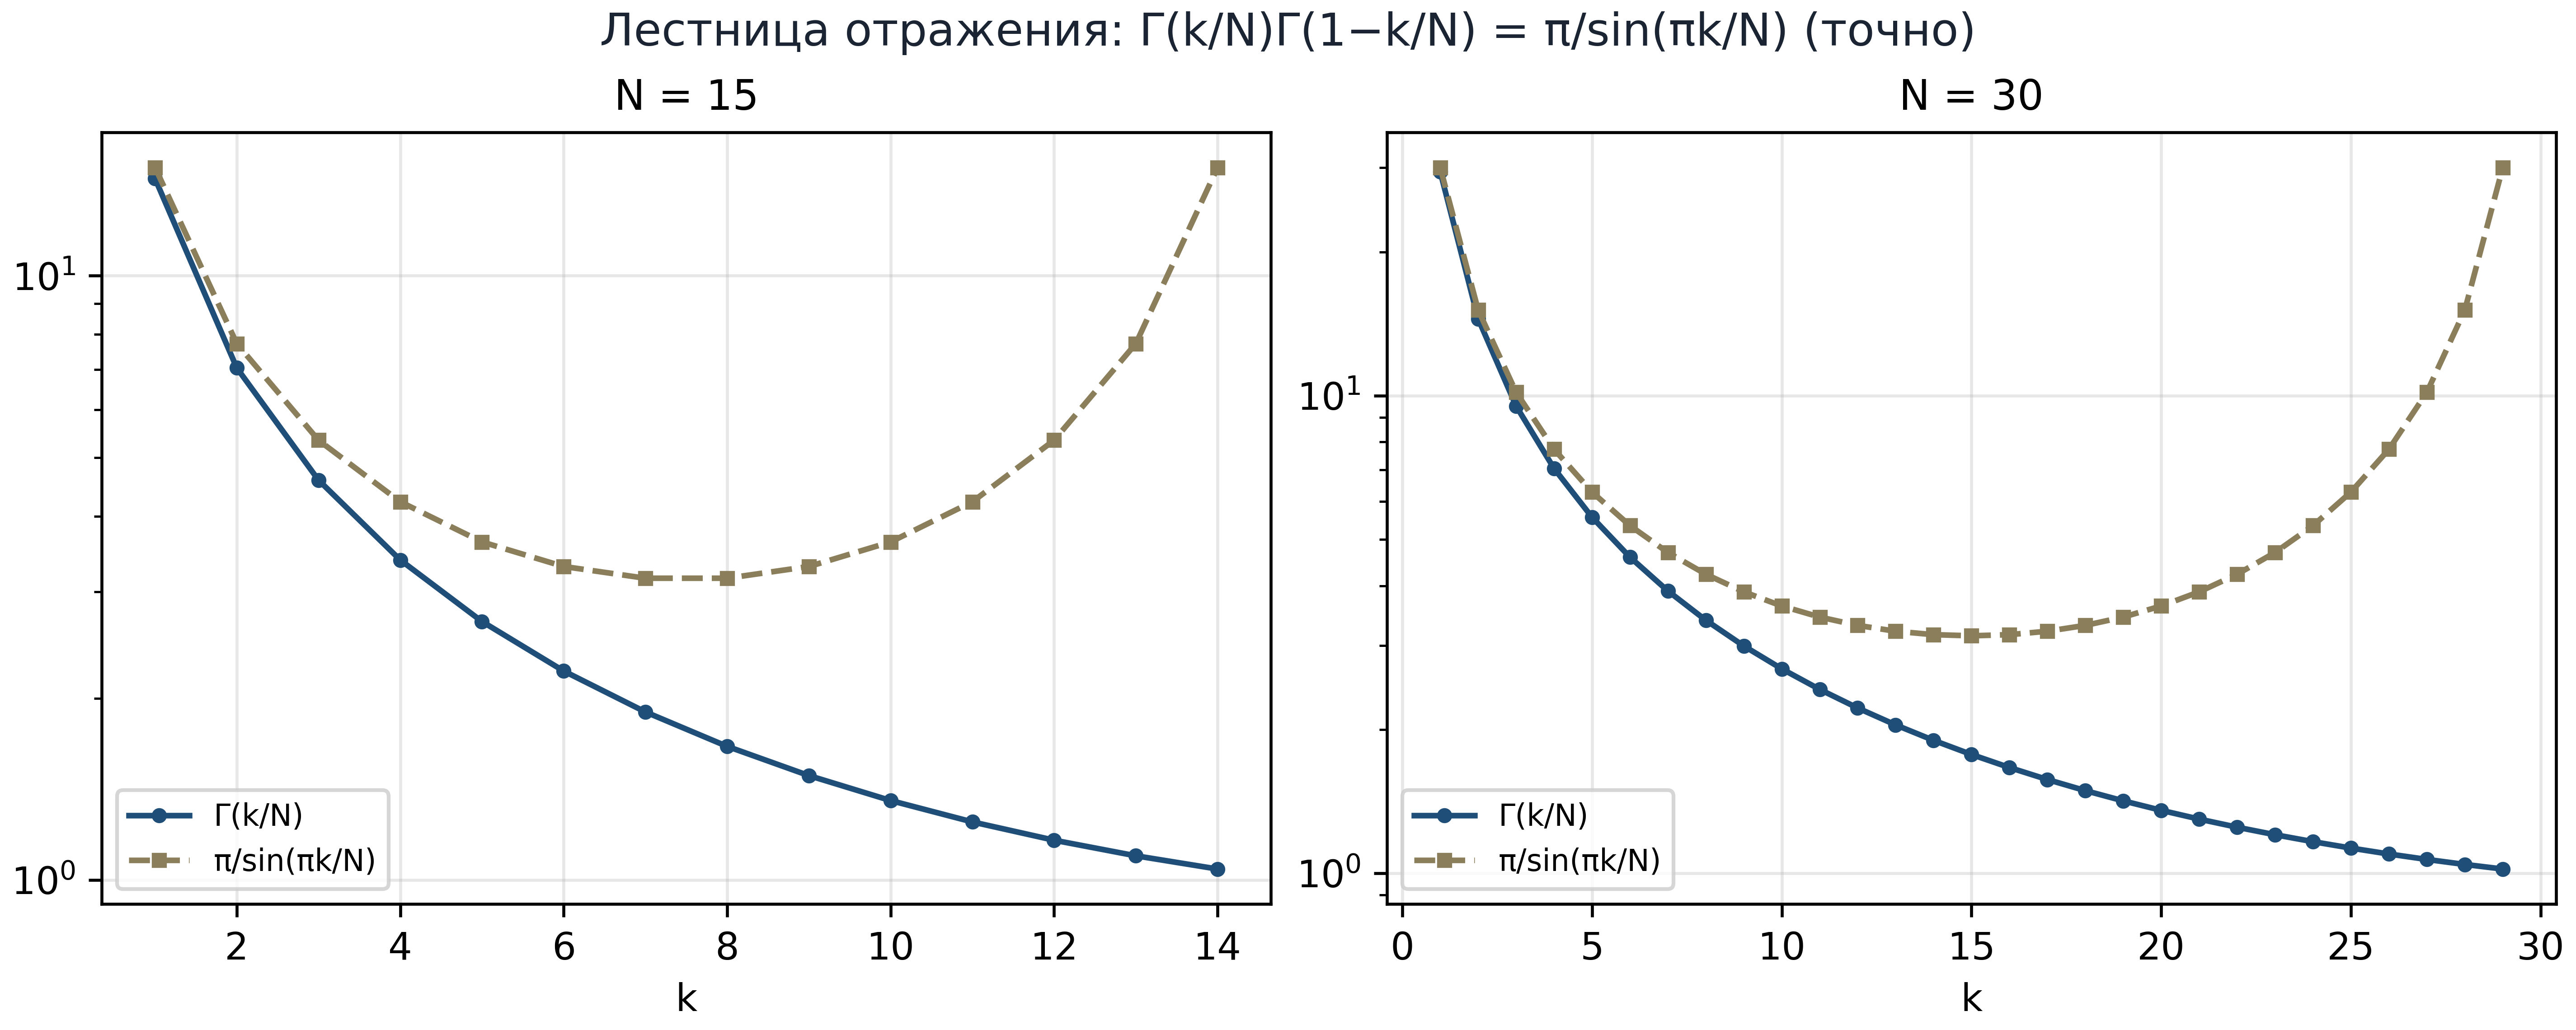
\includegraphics[width=\textwidth]{../ru/figs/fig_gamma.png}
\caption{The reflection ladder: $\Ga(k/N)$ versus
$\pi/\sin(\pi k/N)$ (log scale). The coincidence of the curves at
both levels is the numerical portrait of Lemma~\ref{lem:reflection};
the maximal deviation over all $k$ is $7.0\cdot10^{-36}$ (check V6).}
\label{fig:gamma}
\end{figure}

\begin{figure}[t]
\centering
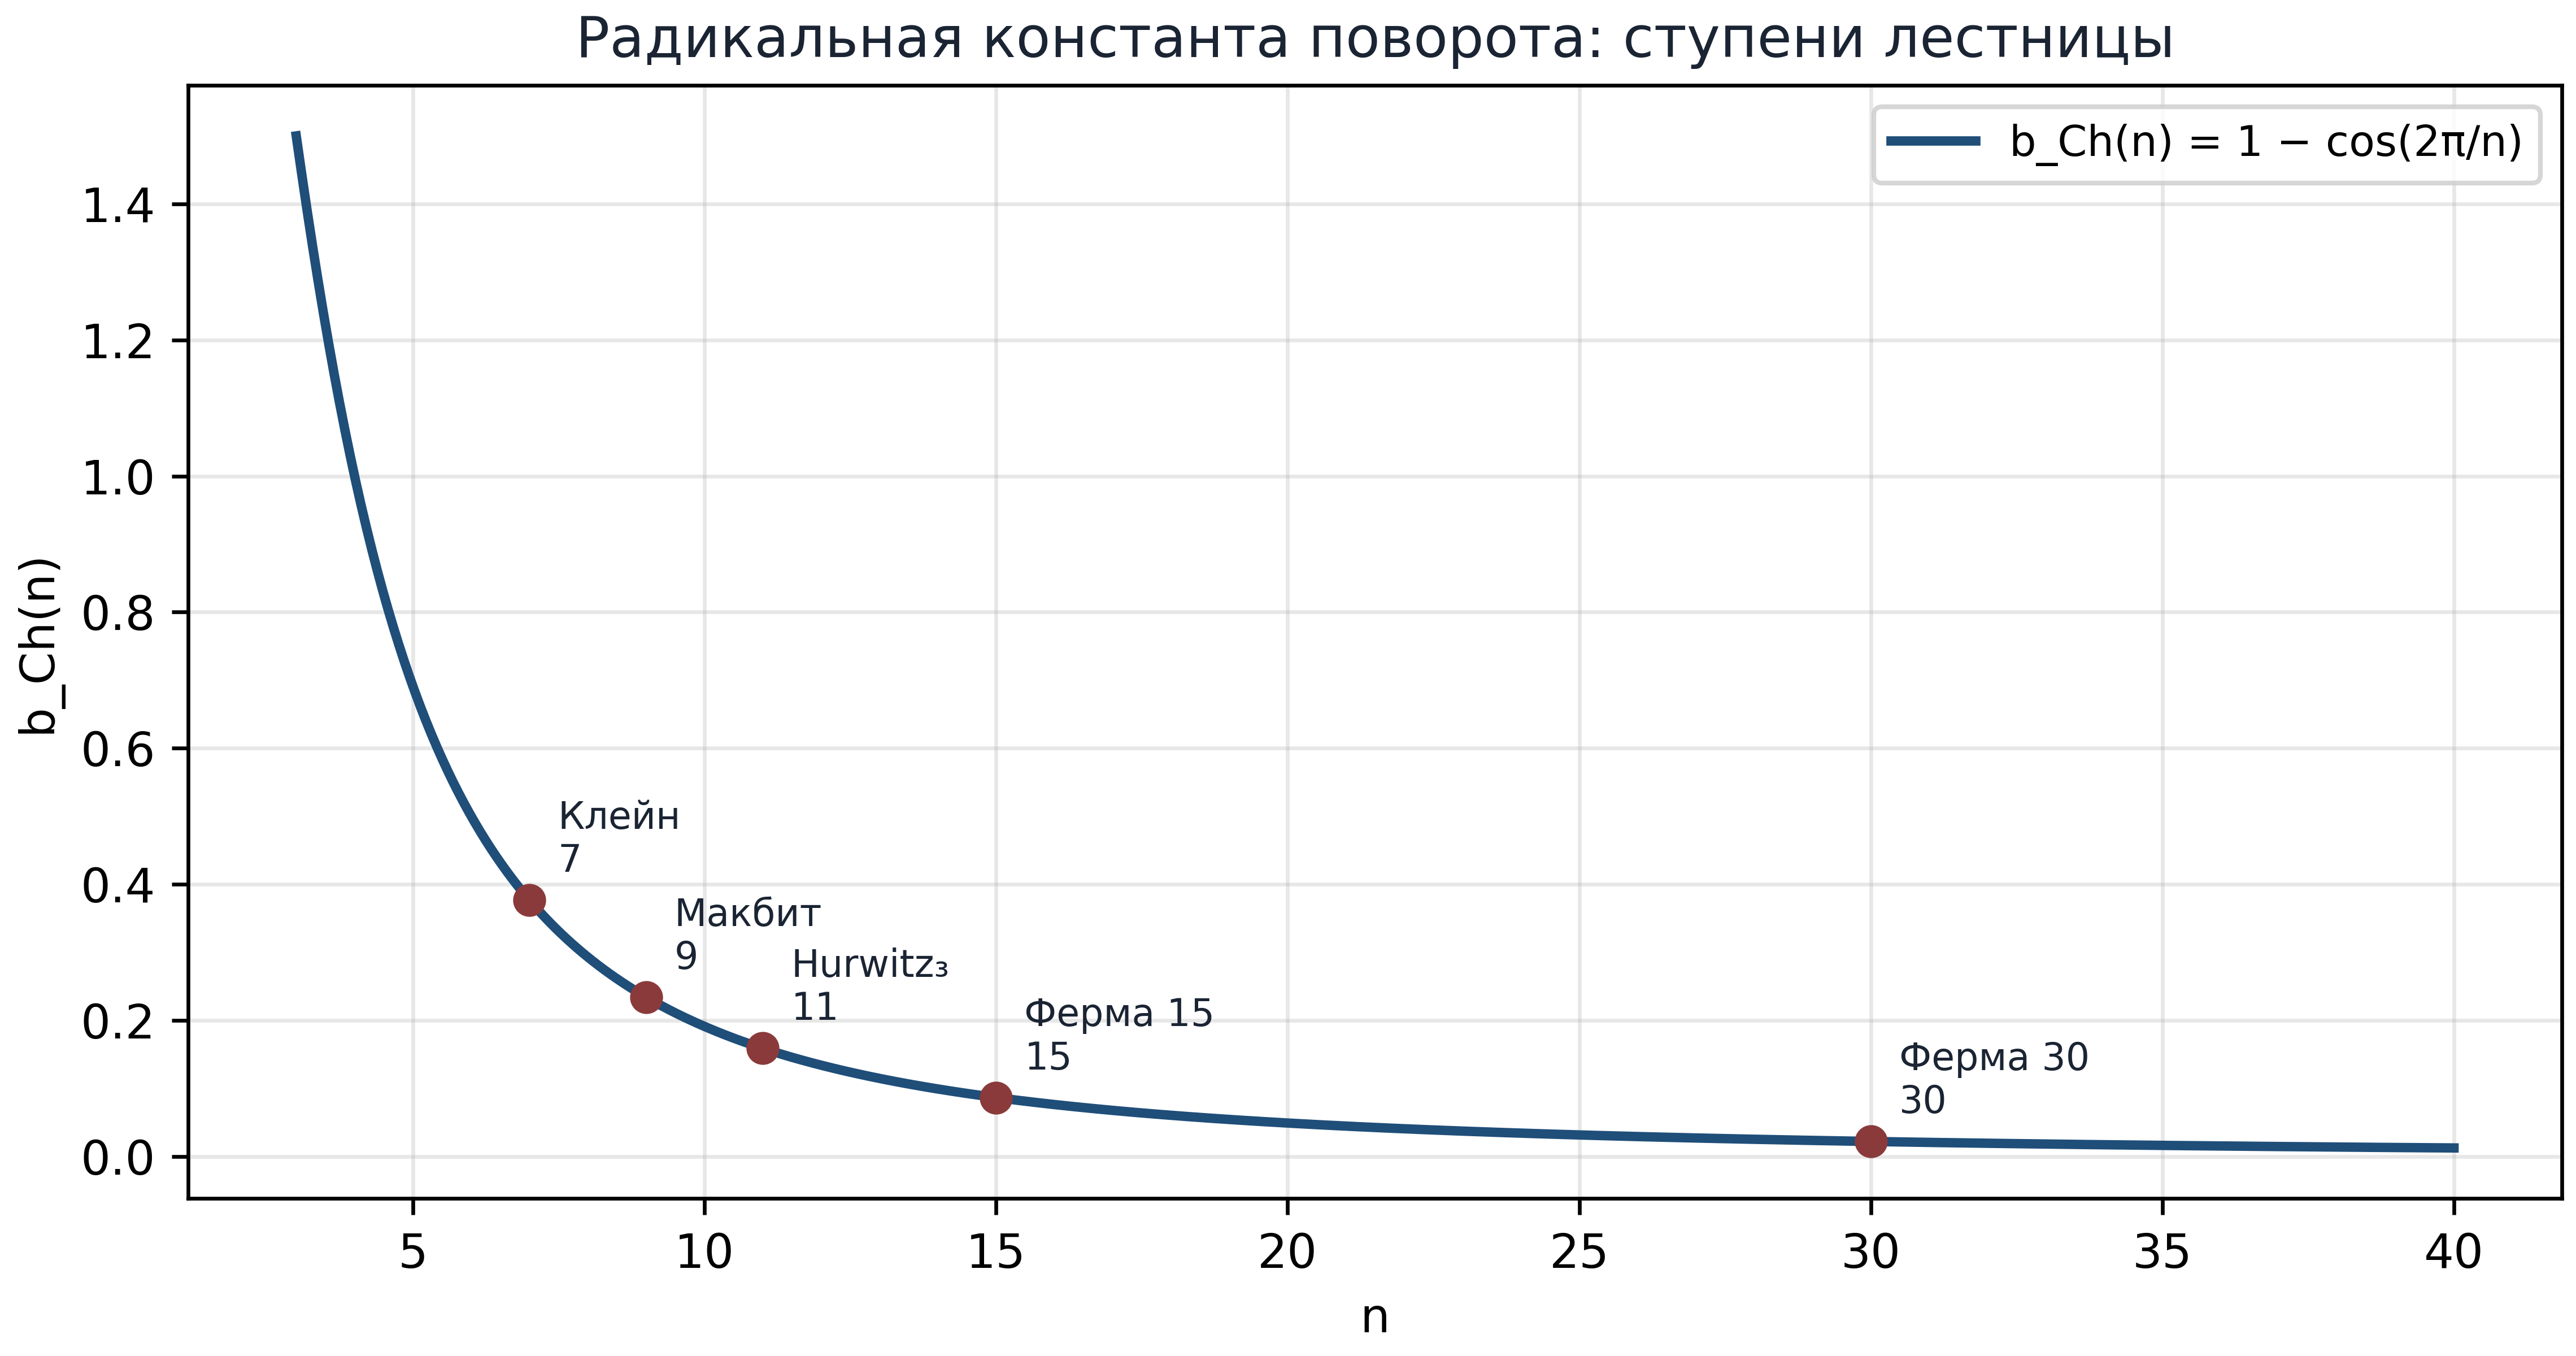
\includegraphics[width=0.82\textwidth]{../ru/figs/fig_bch.png}
\caption{The radical rotation constant $b_{Ch}(n)=1-\cos(2\pi/n)$
with the ladder rungs marked: Klein ($7$), Macbeath ($9$),
Hurwitz$_3$ ($11$), Fermat $15$ and $30$. At the stand levels the
constant takes the exact radical values
\eqref{eq:b15}--\eqref{eq:b30} (Theorem~\ref{th:normalization}).}
\label{fig:bch}
\end{figure}

\begin{figure}[t]
\centering
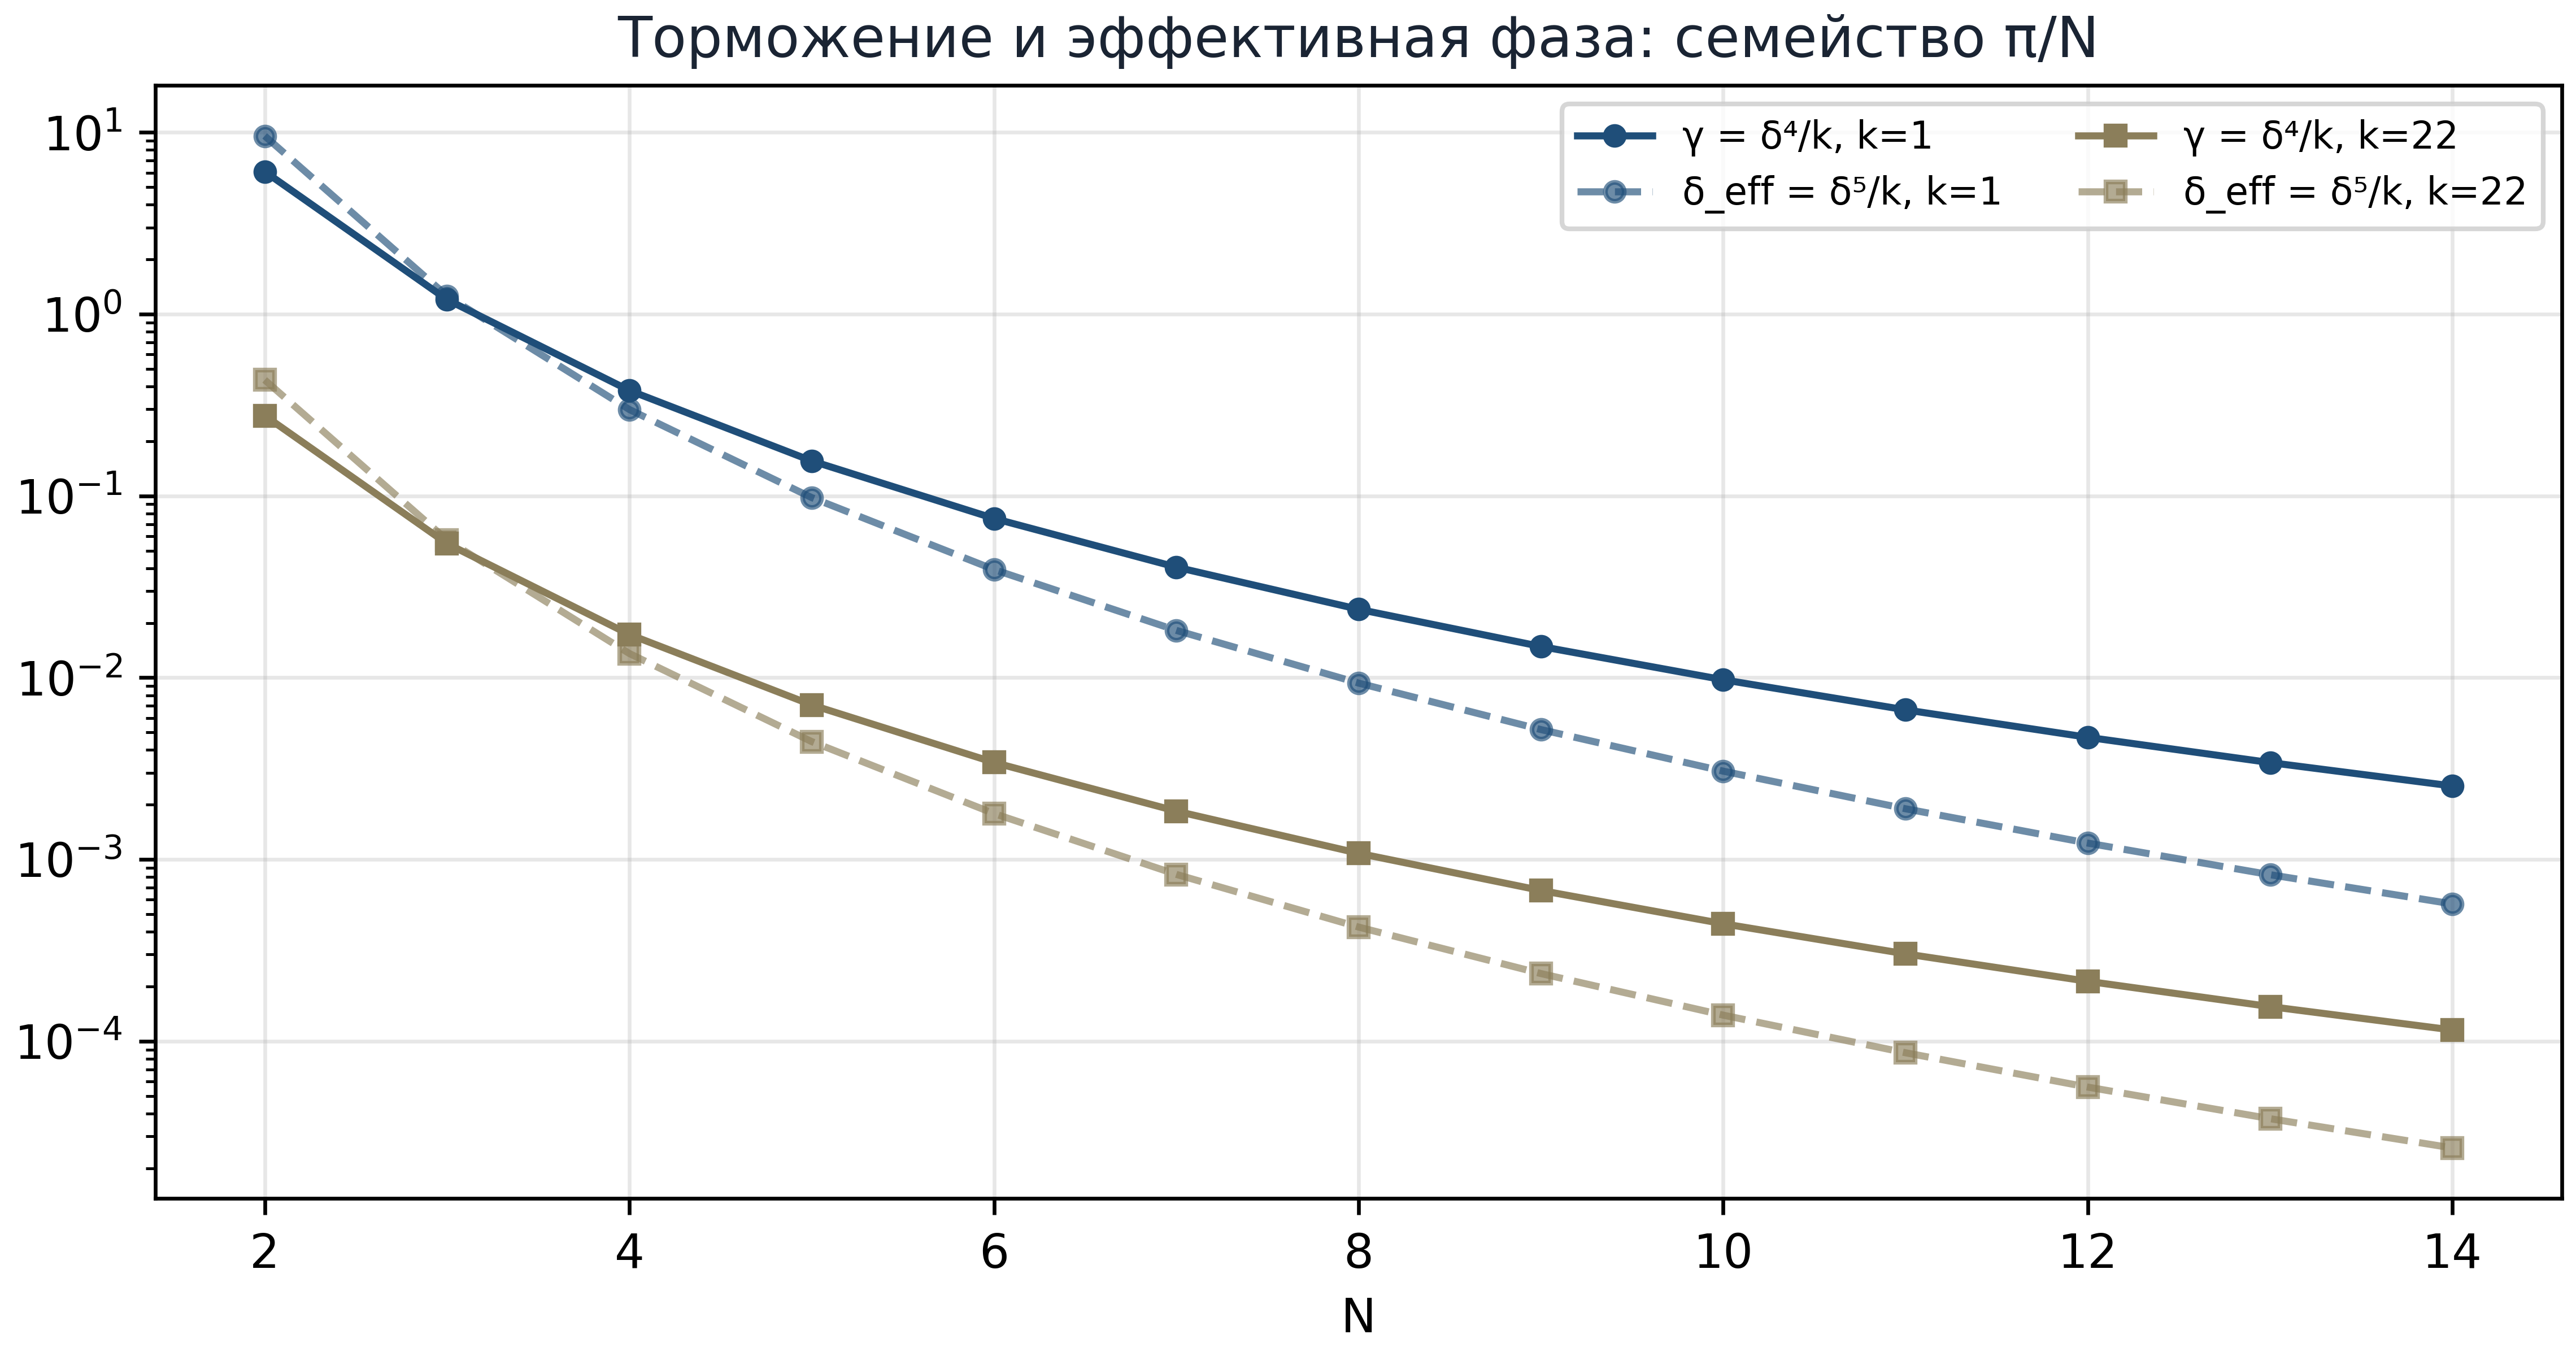
\includegraphics[width=0.82\textwidth]{../ru/figs/fig_torus.png}
\caption{The braking family $\gamma=\delta^4/k$ and effective phases
$\delta_{\mathrm{eff}}=\delta^5/k$ for $k\in\{1,22\}$ --- the two
carriers give two curve families; the carrier $k=22$ suppresses the
correction by two orders of magnitude. Data match
Appendix~\ref{app:fulldata} and Section~\ref{sec:torus}.}
\label{fig:torus}
\end{figure}

\begin{figure}[t]
\centering
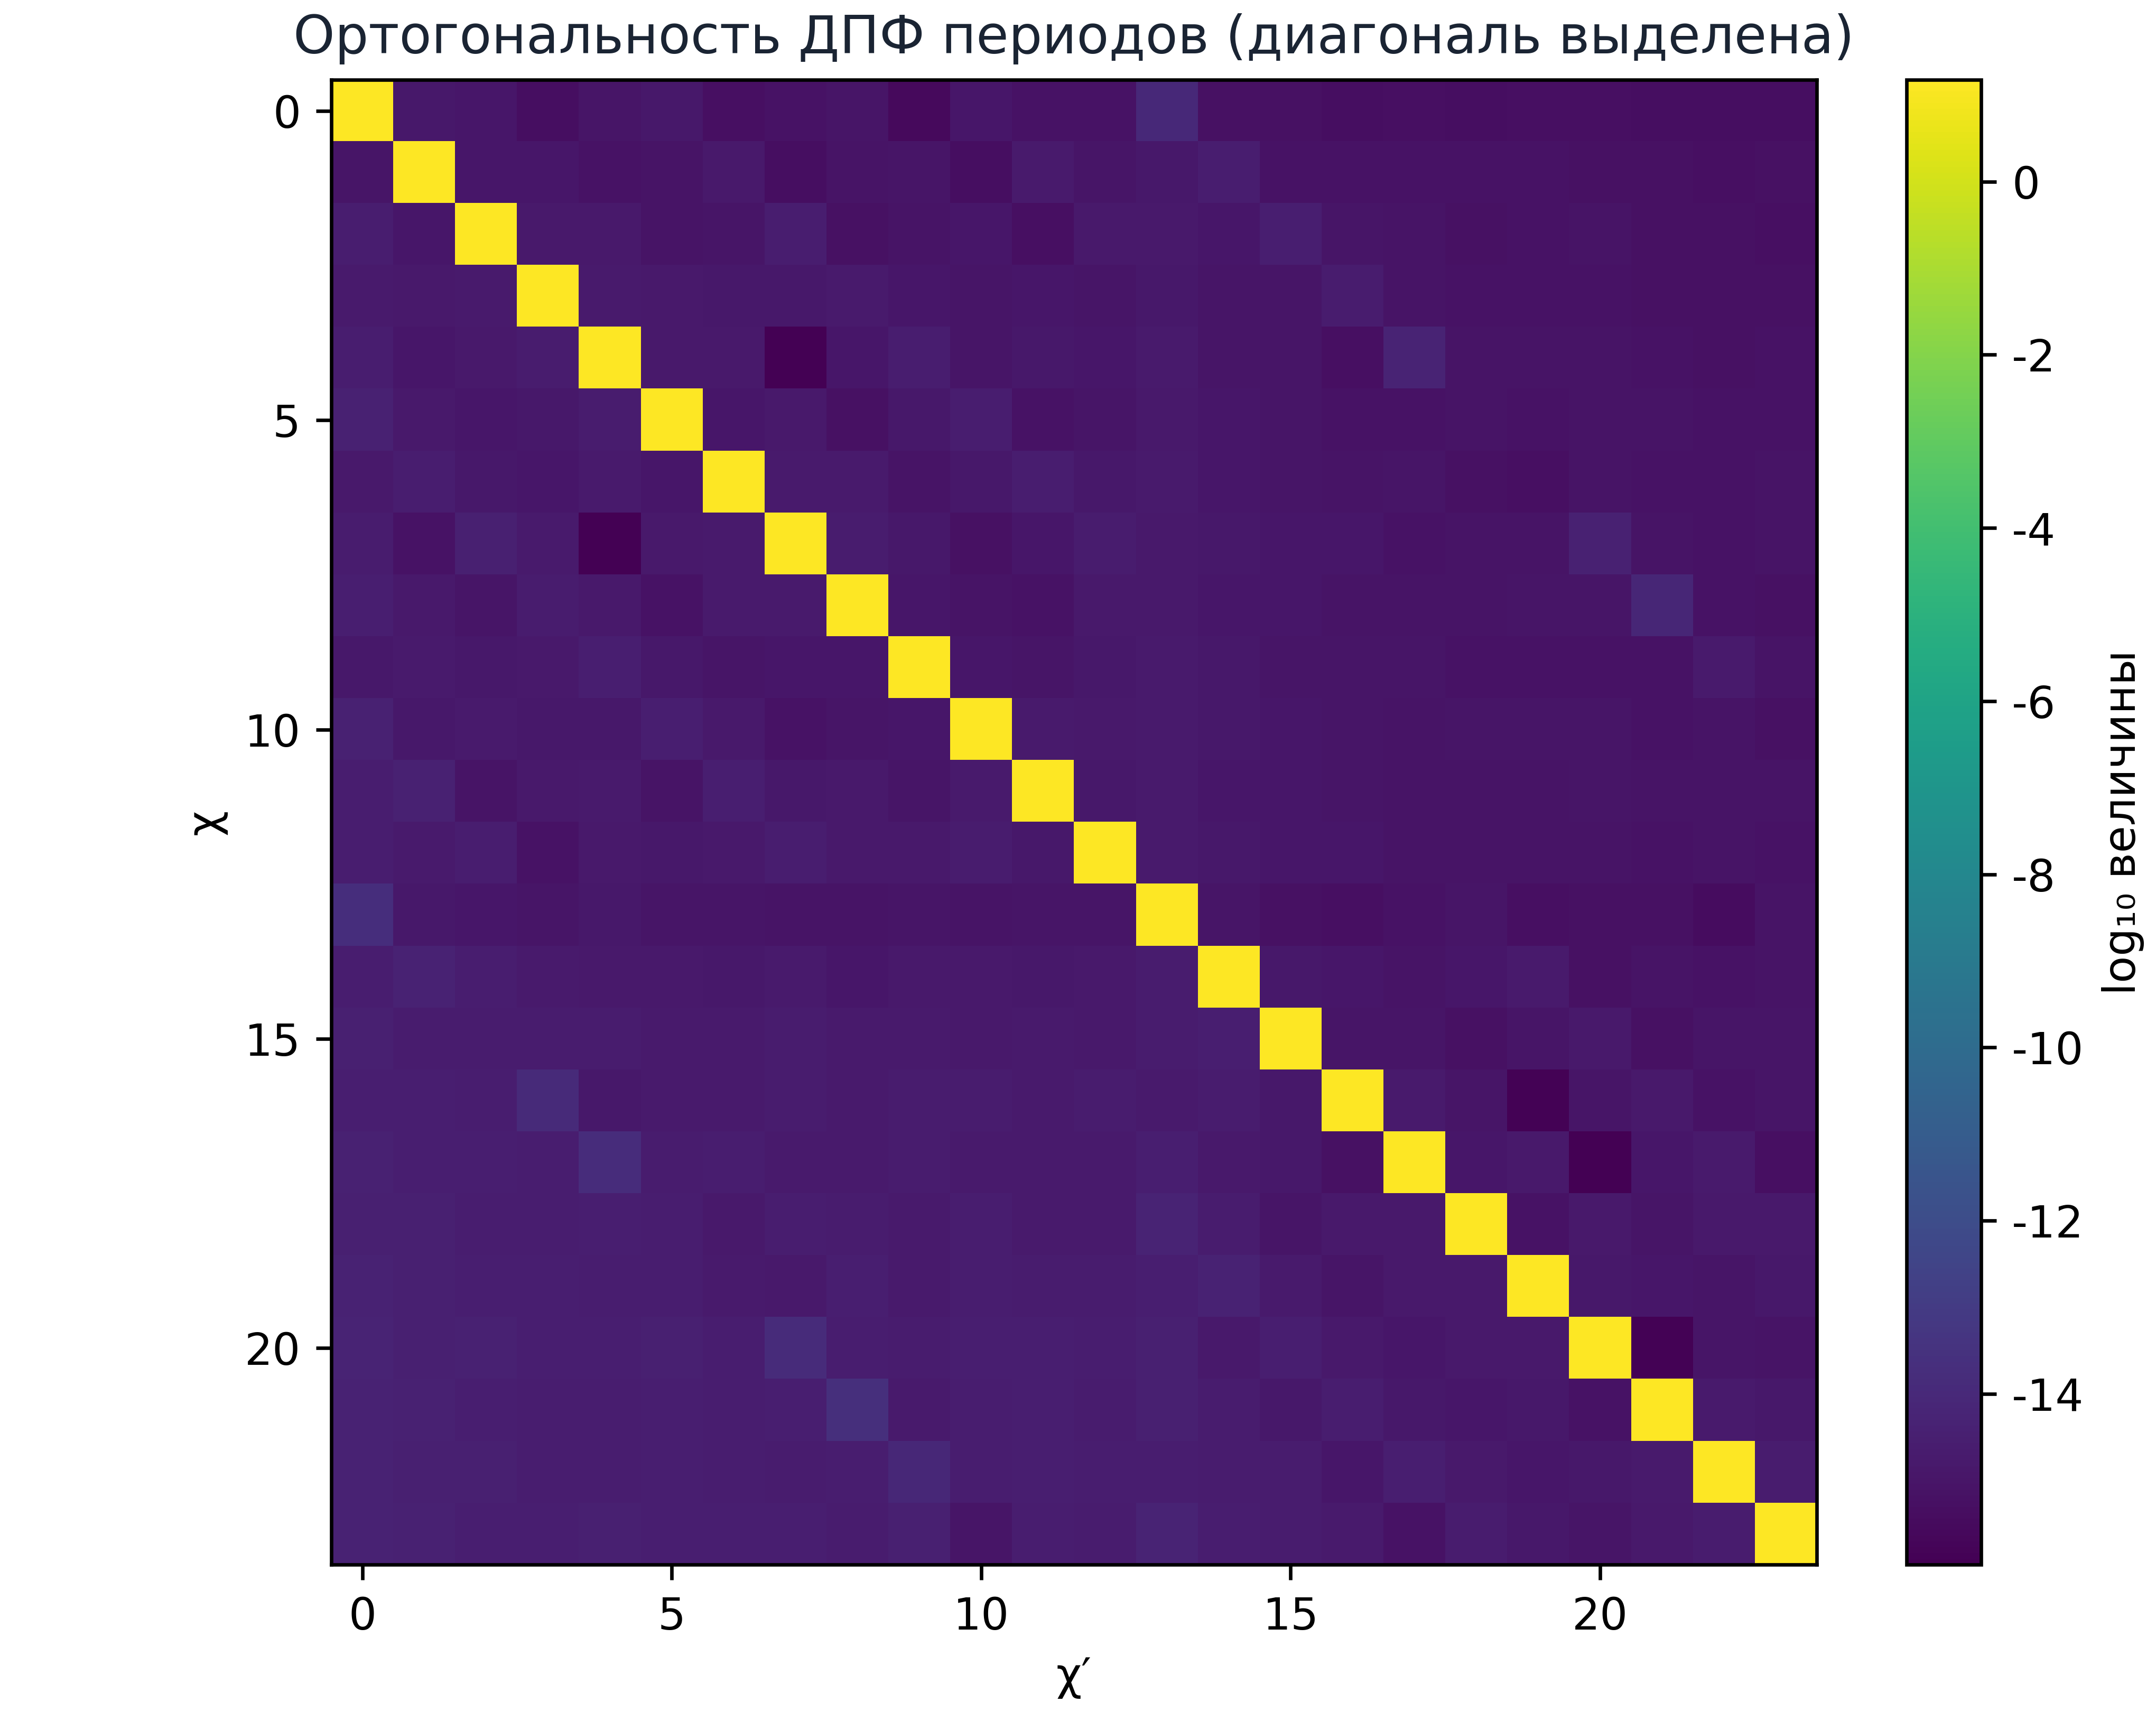
\includegraphics[width=0.78\textwidth]{../ru/figs/fig_dft.png}
\caption{The matrix $|\sum_{r,s}P_\chi\overline{P_{\chi'}}|$ (log
scale): the bright diagonal is $|\Omega_\chi|^2$, the off-diagonal
background at $10^{-37}$ relative to the diagonal is the numerical
portrait of DFT orthogonality (check V8) --- a direct consequence of
the completeness of the character system of $(\ZZ/N)^2$.}
\label{fig:dft}
\end{figure}

\section{The final arch of the program}\label{sec:final}

\emph{The foundation} --- the dynamic principle: geometry supplies
only the integer triple $(n,B,\lambda_0)$; the entire structure is
built by algebra. The principle turns the framework into a pipeline
without free parameters: the spin phase $\pi/N$, the braking
$\delta^4/k$, the effective phase $\delta^5/k$, and the united
formula $\Delta_{Ch}$ --- all derived, all checkable.

\emph{The calibration} --- three stands: the torus with the full
explicit derivation of $(4,1,4\pi^2)$ and exact
$\mu_4$-equivariance; K3 with maximal rank $\rho=20$, signature
$(1,19)$, determinant $64$ --- all over $\QQ$ from the explicit
$49\times49$ matrix; Klein with the heptad arithmetic $\Delta=-7^3$,
$j=-3375$, and the recovery of $j$ from the period with $57$ digits.

\emph{The certificates} --- eight documents A through H: the explicit
divisor, the closure of the kernel $29$ by periods, the equivariance
$22=1+7+7+7$, the universal $\mu_4$ theorem, flow termination with
exact time, rationalization with the a priori bound $Q=256$, Hodge
lattice indices with the Chowla--Selberg layer, and --- the summit
--- the $N=15/30$ stand in the full Gross $\Ga$-normalization: SNF
type $(1,1,5,5,15,15,15,15)$, discriminant $1125^2$, volume
$\mathrm{vol}_h=1125$, denominator bound $480$.

\emph{The closed system} --- the $N=15/30$ stand: eight lemmas and
six theorems with complete proofs, from cycle combinatorics to
polarization and indices; every quantity in closed form, every
identity either proved or certified by independent integration to
$10^{-36}$; the protocol V1--V9 reproduces everything with one
command.

Three features distinguish the program from standard computational
practice. First, \emph{closedness}: no quantity is taken from
outside without a derivation or an independent certificate. Second,
\emph{reproducibility}: the full protocol, five languages, the Lean
kernel --- agreement of independent implementations down to integer
values and machine limits. Third, \emph{portability}: new geometry
enters through the triple, and the pipeline works unchanged --- the
ladder from the torus to $N=30$ is the constructive proof of
portability.

The ladder continues: levels $\pi/N$ with growing $N$, conductor
blocks with growing index counts, matrix towers with growing scale.
The infrastructure --- the laboratory, the certificates, the Lean
panel, the multilingual verification --- is designed so that every
new rung stands on a ready foundation: the experiment designer runs
new configurations without code changes, and the protocol certifies
them by the same rules. In this sense the monograph is not an end
but a foundation: the arch is built, and every new rung gets its
place in a working system.
